% Compile with:
% latexmk -lualatex -pvc -interaction=nonstopmode *.tex
%\documentclass[aspectratio=169,draft]{beamer}
\documentclass[aspectratio=169]{beamer}
\usetheme{UniBern}

\title{Talk title}
\author{David Haberthür}
\date{\today\xspace | \href{https://example.com}{Event}}

%\includeonlyframes{current}
%then....
%\begin{frame}[label=current]
%\end{frame}

\usepackage[mode=match,%determines whether siunitx uses math or text mode when printing output.
	per-mode=symbol,% '/' instead of '^-1'
	]{siunitx}
\usepackage{xspace}
\usepackage{gitinfo2}
\usepackage[style=numeric,
	url=false,
	maxnames=1,
	sorting=none,
	]{biblatex}
\addbibresource{~/P/Documents/library.bib}% anaklin25
\addbibresource{~/Documents/library.bib}% anomalocaris
\usepackage{ccicons}% for \source'ing images
\usepackage{animate}
\usepackage{tikz}
	\usetikzlibrary{shadows,spy,mindmap}
	\tikzset{shadowed/.style={preaction={transform canvas={shift={(1pt,-1pt)}},draw=ubRed}}}
\usepackage{shadowtext}% for the shadowed scalebar
	\shadowoffset{1pt}
	\shadowcolor{ubRed}
\usepackage[absolute,overlay]{textpos}% for the \source* command
\usepackage{fontawesome5}
\usepackage{adjustbox}
\usepackage{lipsum}
\usepackage{microtype}

% Some often used abbreviations and commands
\newcommand{\everyframe}{1}% use only every nth frame for the animations
\newcommand{\imwidth}{\linewidth}% set global image width
\newcommand{\imheight}{0.725\paperheight}% set global image height
\newlength\imagewidth% needed for scalebars
\newlength\imagescale% needed for scalebars
\newcommand{\uct}{\textmu CT\xspace}% make our life easier
\newcommand{\uaf}{\textmu Angiofil\xspace}% make our life easier
\newcommand{\eg}{e.\,g.\xspace}%
\newcommand{\ie}{i.\,e.\xspace}%

% Acknowledge images just below them
% Based on https://tex.stackexchange.com/a/282637/828
\newcommand{\source}[2]{%
	% Print out (short) link under image, with small text
	\raisebox{-1.618ex}{%
		\makebox[0pt][r]{%
			\scriptsize\href{http://#1}{#1} #2%
			}%
		}%
	}%
\newcommand{\sourcecite}[2]{%
	% Cite (an image from) a reference
	\raisebox{-1.618ex}{%
		\makebox[0pt][r]{%
			\scriptsize From \cite{#1}, #2%
			}%
		}%
	}%
\newcommand{\sourcelink}[3]{%
	% Make the source command an \href{link}{text}
	\raisebox{-1.618ex}{%
		\makebox[0pt][r]{%
			\scriptsize\href{http://#1}{#2}, #3%
			}%
		}%
	}%
% Define us a custom footer *with* progress bar, based on https://tex.stackexchange.com/a/59749/828
\makeatletter
\def\progressbar@progressbar{}% the progress bar
\newcount\progressbar@tmpcounta% auxiliary counter
\newcount\progressbar@tmpcountb% auxiliary counter
\newdimen\progressbar@pbht%progressbar height
\newdimen\progressbar@pbwd%progressbar width
\newdimen\progressbar@rcircle% radius for the circle
\newdimen\progressbar@tmpdim% auxiliary dimension
\progressbar@pbwd=0.8\linewidth
\progressbar@rcircle=1.5pt
\def\progressbar@progressbar{%
	\progressbar@tmpcounta=\insertframenumber%
	\progressbar@tmpcountb=\inserttotalframenumber%
	\progressbar@tmpdim=\progressbar@pbwd%
	\multiply\progressbar@tmpdim by \progressbar@tmpcounta%
	\divide\progressbar@tmpdim by \progressbar@tmpcountb%
	\par%
	\hfill%
	\begin{tikzpicture}%
		\draw[ubGrey] (0,0) -- ++ (\progressbar@pbwd,0);
		\draw[draw=ubRed,fill=ubGrey] (\the\dimexpr\progressbar@tmpdim-\progressbar@rcircle\relax,.5\progressbar@pbht) circle (\progressbar@rcircle);
	\end{tikzpicture}%
	\hfill\xspace|\xspace\$Link%
	\hfill\xspace|\xspace v.~\href{https://github.com/habi/$CHANGE_TO_CORRECT_REPOSITORY/commit/\gitHash}{\gitAbbrevHash}%
	\hfill\xspace|\xspace p.~\insertframenumber/\inserttotalframenumber%
	\hfill%
%	\hspace*{4ex}%
	\vspace{0.5ex}%
	\par%
}
\addtobeamertemplate{footline}{}%
{%
	\begin{beamercolorbox}[wd=\paperwidth,center]{ubRed}%
		\progressbar@progressbar%
	\end{beamercolorbox}%
}%
\makeatother

% Format bibliography for beamer
% http://tex.stackexchange.com/a/10686/828
\renewbibmacro{in:}{}
% http://tex.stackexchange.com/a/13076/828
\AtEveryBibitem{%
	\clearfield{journaltitle}
	\clearfield{pages}
	\clearfield{volume}
	\clearfield{number}
	\clearname{editor}
	\clearfield{issn}
	\clearfield{year}
}
% No parentheses around the (now empty) year: https://tex.stackexchange.com/a/147537/828
\renewcommand{\bibopenparen}{\addcomma\addspace}
\renewcommand{\bibcloseparen}{\addcomma\addspace}

% open in fullscreen automatically
%\hypersetup{pdfpagemode=FullScreen}

% Move the whole text area down a bit
% THIS IS A BIG HACK, AND SHOULD BE FIXED IN THE TEMPLATE
\addtobeamertemplate{frametitle}{}{\vspace*{0.71em}}

\begin{document}
% No footline on the title page
% http://tex.stackexchange.com/a/18829/828 helps us to achieve that
{%
	\setbeamertemplate{footline}{}%
	\begin{frame}%
		\maketitle
	\end{frame}%
}

\begin{frame}
	\frametitle{Alignment frame}
	\tiny\lipsum[1-5]
\end{frame}

\begin{frame}
	\frametitle{\emph{Grüessech} from the \uct-group}
	\centering%
	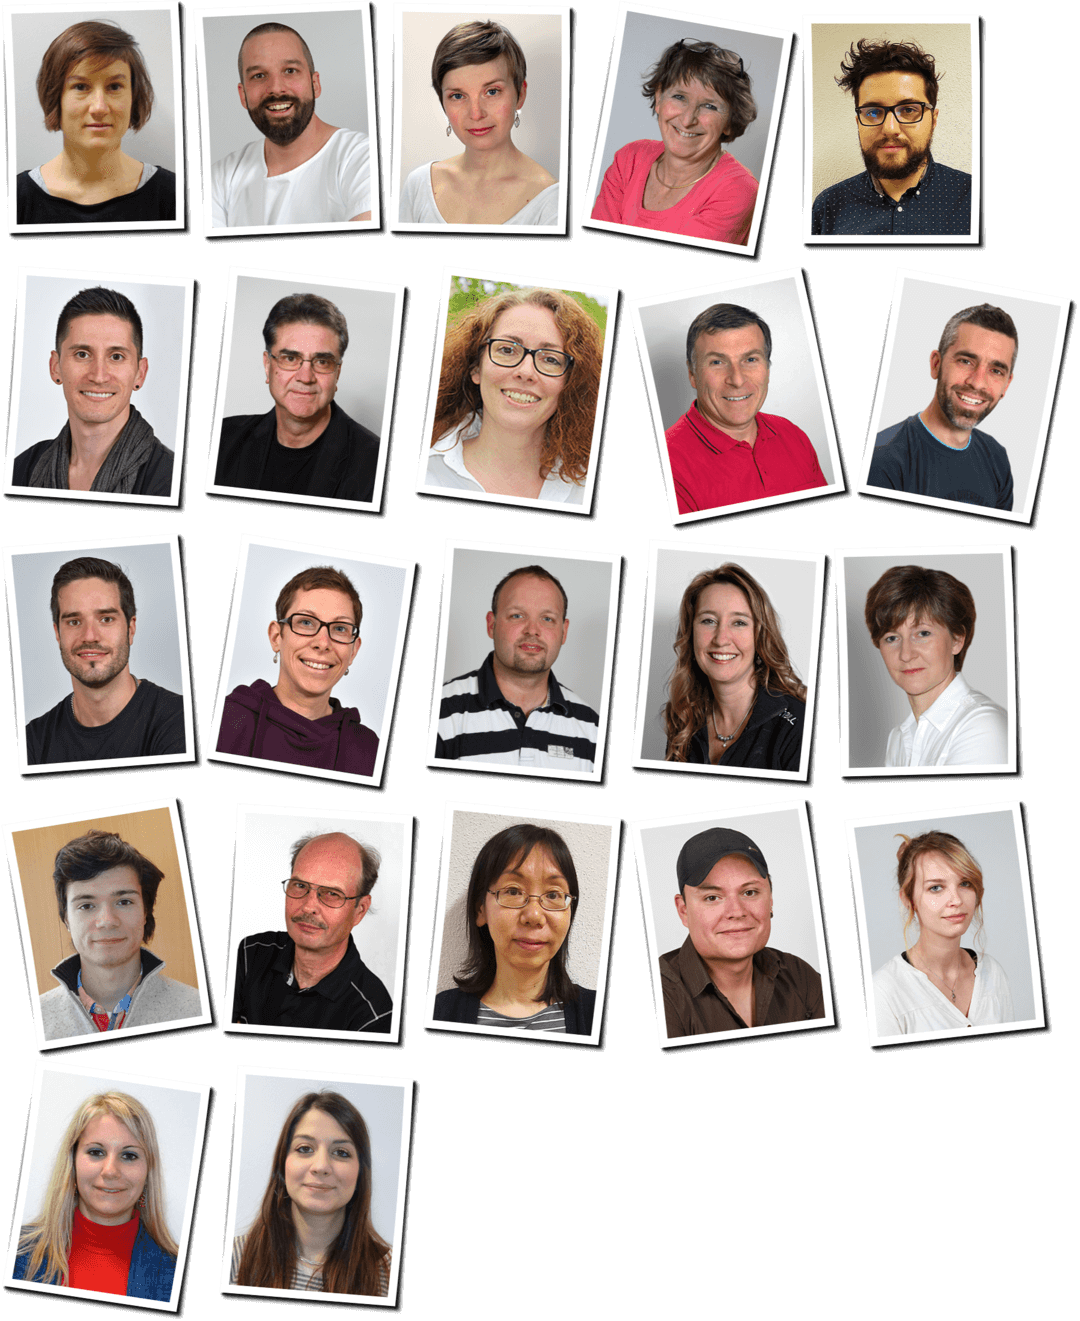
\includegraphics[width=0.85\linewidth]{./img/team}%
	\begin{columns}%
		\hfill
		\begin{column}{0.3\linewidth}
			\centering%
			David{\color{ubRed!50}.}%
			\only<1>{Haberthür{\color{ubRed!50}@unibe.ch}}%
			\only<2>{Haberthuer{\color{ubRed!50}@unibe.ch}}
		\end{column}
		\begin{column}{0.3\linewidth}
			\centering%
			Ruslan{\color{ubRed!50}.}Hlushchuk{\color{ubRed!50}@unibe.ch}%
		\end{column}
		\begin{column}{0.3\linewidth}
			\centering%
			Oleksiy{\color{ubRed!50}.}Khoma{\color{ubRed!50}@unibe.ch}%
		\end{column}%
	\hfill%
	\end{columns}
\end{frame}

\begin{frame}
	\frametitle{Overview}
	\begin{columns}
		\begin{column}{0.33\linewidth}
			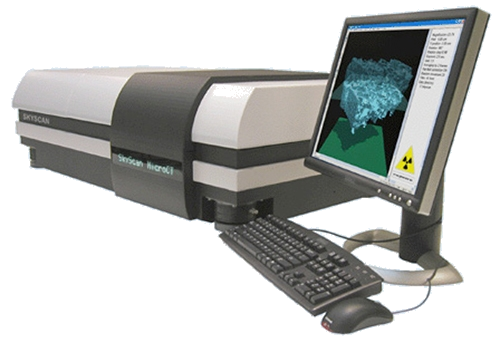
\includegraphics[width=\linewidth]{./img/1172}%
			\sourcelink{tissueengineering.no/wp-content/uploads/2020/10/SKyscan-1172.jpg}{Bruker SkyScan 1172}{}%
		\end{column}
		\begin{column}{0.33\linewidth}
			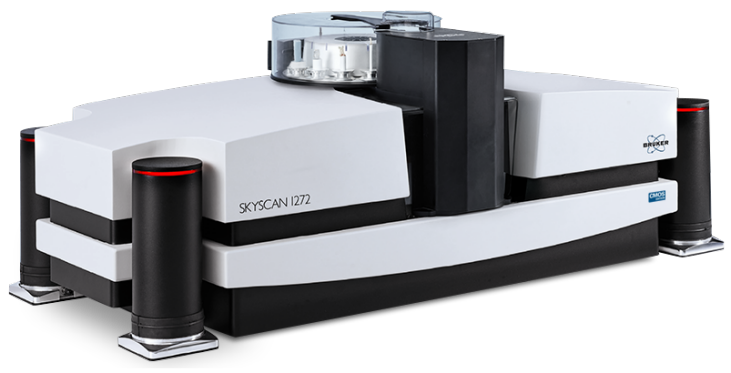
\includegraphics[width=\linewidth]{./img/1272}%
			\sourcelink{bruker.com/skyscan1272}{Bruker SkyScan 1272}{}%
		\end{column}
		\begin{column}{0.33\linewidth}
			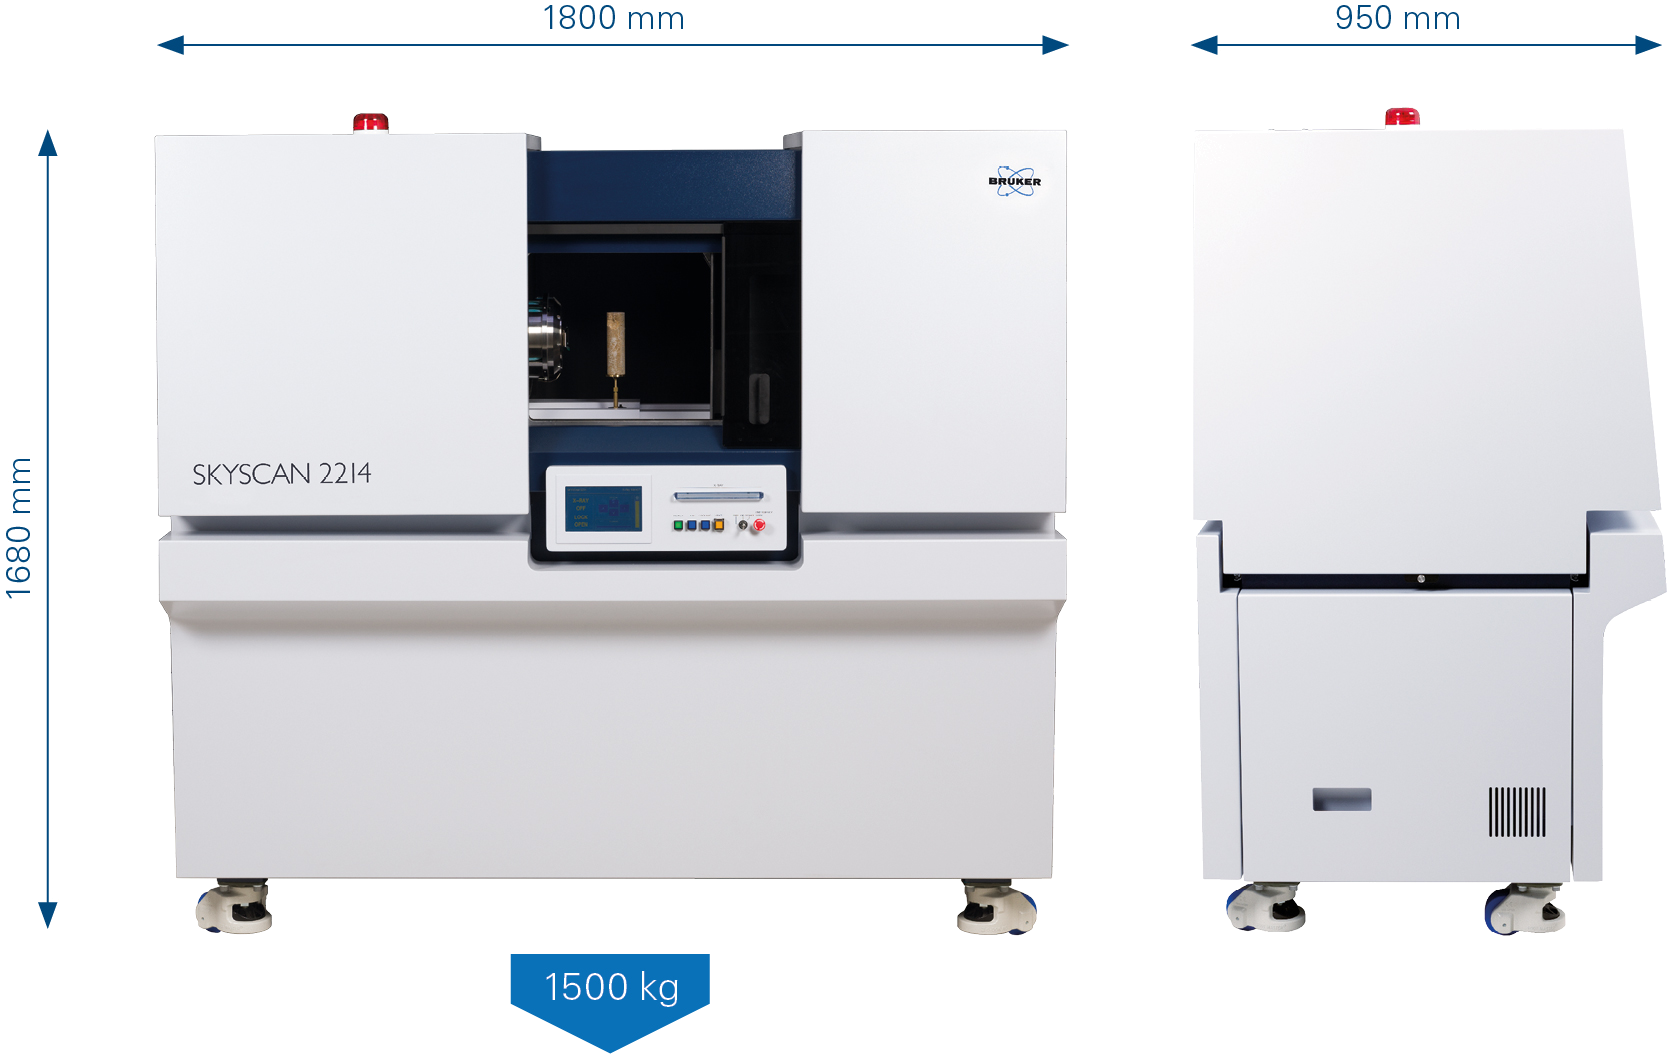
\includegraphics[width=\linewidth]{./img/2214}%
			\sourcelink{bruker.com/skyscan2214}{Bruker SkyScan 2214}{}%
		\end{column}
	\end{columns}
\end{frame}

\begin{frame}
	\frametitle{Thanks}
	\begin{columns}
		\begin{column}{0.495\linewidth}
			\begin{itemize}
				\item All the collaborators, for collaborating
				\item SNF, for paying my wages
				\item<2-> You, for listening to me%
			\end{itemize}%
		\end{column}
		\begin{column}{0.495\linewidth}
			\centering
			Let's show a nice image here
		\end{column}
	\end{columns}	
\end{frame}

\begin{frame}
	\frametitle{References}
	% Make the references continuously smaller :)
	%\renewcommand*{\bibfont}{\small}
	%\renewcommand*{\bibfont}{\footnotesize}
	%\renewcommand*{\bibfont}{\scriptsize}
	%\renewcommand*{\bibfont}{\tiny}
%	\setbeamertemplate{bibliography item}{\insertbiblabel}
	\printbibliography
\end{frame}

\end{document}

